\documentclass[9pt,twocolumn,twoside]{gsag3jnl}
% Use the documentclass option 'lineno' to view line numbers

\articletype{gos} % article type
% {inv} Investigation
% {gs} Genomic Selection
% {goi} Genetics of Immunity
% {gos} Genetics of Sex
% {mp} Multiparental Populations
\usepackage{gensymb}
\usepackage[switch]{lineno}
\usepackage{siunitx}


% new commands
\newcommand{\cel}{\emph{C.~elegans}}
\newcommand{\fog}{\emph{\mbox{fog-2(lf)}}}
\newcommand{\gene}[1]{\emph{\mbox{#1}}}
\newcommand{\ecol}{\emph{E.~coli}}

% gene numbers
\newcommand{\fogn}{1,881}
\newcommand{\agen}{5,592}
\newcommand{\interactionn}{1,318}
\newcommand{\coexpressed}{905}
\newcommand{\intersectn}{1,040}
\newcommand{\femalen}{405}

% tf numbers
\newcommand{\tfaging}{145}
\newcommand{\tffog}{60}
\newcommand{\tfinteraction}{36}

% number of genes in gold standard
\newcommand{\goldn}{1,056}
\newcommand{\goldfound}{506}
\newcommand{\goldpval}{$<10^{-38}$}

% website commands
\newcommand{\website}{
            \url{https://wormlabcaltech.github.io/Angeles_Leighton_2016}
            }
\newcommand{\webref}{
\href{https://wormlabcaltech.github.io/Angeles_Leighton_2016}{website}}

\newcommand{\titleone}{The \cel{} female state: Decoupling the
transcriptomic effects of aging and sperm-status}

\title{\titleone}

\author[$\ast$, \S]{David Angeles-Albores}
\author[$\ast,\dagger$, \S]{Daniel H.W. Leighton}
\author[$\ast$]{Tiffany Tsou}
\author[$\ast$]{Tiffany H. Khaw}
\author[$\ddagger$]{Igor Antoshechkin}
\author[$\ast$, 1]{Paul W. Sternberg}

\affil[$\ast$]{Department of Biology and Biological Engineering,
and Howard Hughes Medical Institute, Caltech, Pasadena, CA, 91125, USA}
\affil[$\dagger$]{Current:Department of Human Genetics, Department of Biological
Chemistry, and Howard Hughes Medical Institute, University of California,
Los Angeles, Los Angeles, CA 90095, USA}
\affil[$\ddagger$]{Department of Biology and Biological Engineering, Caltech,
Pasadena, CA, 91125, USA}
\affil[$\S$]{These authors contributed equally to this work}

\keywords{epistasis; genetic interactions; ageing; life cycle; RNA-seq; germline
sex determination}

\runningtitle{The \cel{} female-like state} % For use in the footer

\correspondingauthor{Angeles-Albores}
\linenumbers{}

\begin{abstract}
  % Understanding genome and gene function in a whole organism requires us to
  % fully comprehend the life cycle and the physiology of the organism in question.
  % Although \cel{} is traditionally thought of as a hermaphrodite, XX animals exhaust
  % their sperm and become endogenous females after 3 days of egg-laying.
  % The molecular physiology of this state has not been as intensely studied as other
  % parts of the life cycle, despite documented changes in behavior and metabolism
  % that occur at this stage. To study the female-like state of \cel{}, we measured the
  % transcriptomes of 1st day adult hermaphrodites; endogenous, 6th day adult females;
  % and at the same time points, mutant \fog{} worms that have a feminized germline
  % phenotype. At these time points, we could separate the effects of biological
  % aging from the transition into the female-like state.\@ \fog{} mutants partially phenocopy
  % 6 day adult wild-type animals and exhibit fewer differentially expressed genes as
  % they age throughout these 6 days. Therefore, \emph{fog-2} is epistatic to age as
  % assessed by this transcriptomic phenotype, which indicates that both factors act
  % on sperm status to mediate entry into the female-like state. These changes are enriched
  % in transcription factors canonically associated with neuronal development and
  % differentiation. Our data provide a high-quality picture of the changes that
  % happen in global gene expression throughout the period of early aging in the
  % worm.
  Understanding genome and gene function in a whole organism requires us to
  fully comprehend the life cycle and the physiology of the organism in
  question. \emph{Caenorhabditis~elegans} XX animals are hermaphrodites that
  exhaust their sperm after 3 days of egg-laying. Even though \cel{} can live
  for many days after cessation of egg-laying, the molecular physiology of this
  state has not been as intensely studied as other parts of the life cycle,
  despite documented changes in behavior and metabolism. To study the effects of
  sperm depletion and aging of \cel{} during the first 6 days of adulthood, we
  measured the transcriptomes of 1st day adult hermaphrodites; 6th day
  sperm-depleted adults; and at the same time points, mutant \fog{} worms that
  have a feminized germline phenotype. We found that we could separate the
  effects of biological aging from sperm depletion. For a large subset of genes,
  young adult \fog{} animals had the same gene expression changes as
  sperm-depleted 6th day wild-type hermaphrodites, and these genes did not
  change expression when \fog{} females reached the 6th day of adulthood. Taken
  together, this indicates that changing sperm status causes a change in the
  internal state of the worm, which we call the female-like state. Our data
  provide a high-quality picture of the changes that happen in global gene
  expression throughout the period of early aging in the worm.

\end{abstract}

\setboolean{displaycopyright}{true}

\begin{document}

\maketitle
\thispagestyle{firststyle}
\marginmark{}
\firstpagefootnote{}
\correspondingauthoraffiliation{Division of Biology and Biological Engineering,
Caltech, 1200 E California Blvd, Pasadena CA 91125
Contact: pws@caltech.edu}
\vspace{-11pt}%

Transcriptome analysis by RNA-seq~\citep{Mortazavi2008} has allowed for in-depth
analysis of gene expression changes between life stages and environmental
conditions in many species~\citep{Gerstein2014,Blaxter2012}.
\emph{Caenorhabditis~elegans}, a genetic model nematode with extremely
well defined and largely invariant development~\citep{Sulston1977,Sulston1983},
has been subjected to extensive transcriptomic analysis across all stages of
larval development~\citep{Hillier2009,Boeck2016,Murray2012}
and many stages of embryonic development~\citep{Boeck2016}. Although RNA-seq was
used to develop transcriptional profiles of the mammalian aging process soon
after its invention~\citep{Magalhaes2010}, few such studies have been conducted
in \cel{} past the entrance into adulthood.

A distinct challenge to the study of aging transcriptomes in \cel{} is the
hermaphroditic lifestyle of wild-type individuals of this species. Young adult
hermaphrodites are capable of self-fertilization~\citep{Brenner1974,Corsi2015},
and the resulting embryos will contribute RNA to whole-organism RNA extractions.
Most previous attempts to study the \cel{} aging transcriptome have addressed
the aging process only indirectly, or relied on the use of genetically or
chemically sterilized animals to avoid this problem~\citep{Murphy2003,
Halaschek-wiener2005,Lund2002,McCormick2012,Eckley2013,Boeck2016,Rangaraju2015}.
In addition, most of these studies obtained transcriptomes using microarrays,
which are less accurate than RNA-seq, especially for genes expressed at low
levels~\citep{Wang2014}.

Here, we investigate what we argue is a distinct state in the \cel{} life cycle.
% the endogenous female-like state.
Although \cel{} hermaphrodites emerge into adulthood replete with sperm,
after about 3 days of egg-laying the animals become sperm-depleted and can only
reproduce by mating. This marks a transition into what we define as the
endogenous female-like state. This state is behaviorally distinguished by
increased male-mating success~\citep{Garcia2007}, which may be due to an
increased attractiveness to males~\citep{Morsci2011}. This increased
attractiveness acts at least partially through production of volatile chemical
cues~\citep{Leighton2014}. These behavioral changes are also coincident with
functional deterioration of the germline~\citep{Andux2008},
muscle~\citep{Herndon2002}, intestine~\citep{McGee2011} and nervous
system~\citep{Liu2013}, changes traditionally attributed to the aging
process~\citep{Golden2007}.

To decouple the effects of aging and sperm-loss, we devised a two factor
experiment. We examined wild-type XX animals at the beginning of adulthood
(before worms contained embryos, referred to as 1st day adults) and after sperm
depletion (6 days after the last molt, which we term 6th day adults). Second, we
examined feminized XX animals that fail to produce sperm but are fully fertile
if supplied sperm by mating with males (see Fig.~\ref{fig:wormlife}). We used
\fog{} mutants to obtain feminized animals. \gene{fog-2} is involved in
germ-cell sex determination in the hermaphrodite worm and is required for sperm
production~\citep{Schedl1988,Clifford2000}. \cel{} defective in sperm formation
will emerge from the larval stage as female adults. As time moves forward, these
spermless worms only exhibit changes related to biological aging. As a result,
\fog{} mutants should show fewer gene changes during the first 6 days of
adulthood compared to their egg-laying counterparts that age and also transition
from egg-laying into a sperm depleted stage.

% We also reasoned that we might be able to
% identify gene expression changes due to different life histories: whereas
% hermaphrodites lay almost 300 eggs over three days, spermless females do not lay
% a single one. The different life histories could affect gene expression.

Here, we show that we can detect a transcriptional signature associated both
with loss of hermaphroditic sperm marking entrance into the endogenous
female-like state. We can also detect changes associated specifically with
biological aging. Biological aging causes transcriptomic changes consisting of
\agen{} genes in \cel{}. 4,552 of these changes occur in both genotypes we
studied, indicating they do not depend on sperm status. To facilitate
exploration of the data, we have generated a website where we have deposited
additional graphics, as well as all of the code used to generate these analyses:
\website{}.

% figure experiment design
\begin{figure}[htbp]
  \renewcommand{\familydefault}{\sfdefault}\normalfont{}
  \centering
  \captionsetup{width=\linewidth}
  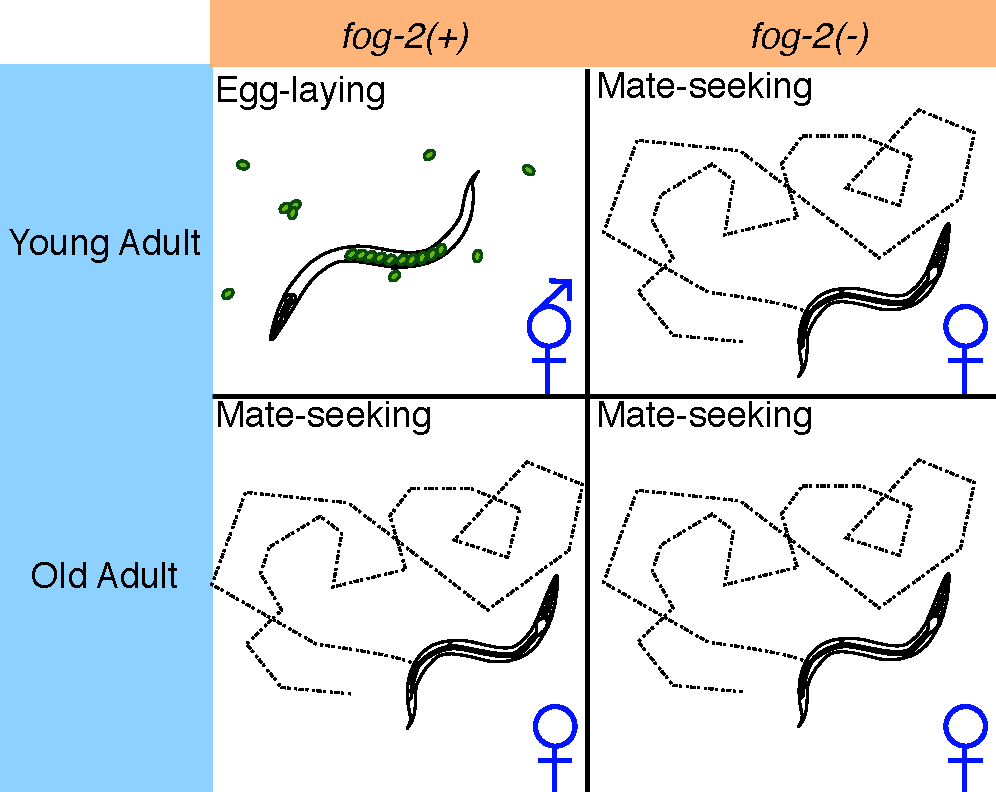
\includegraphics[width=0.6\linewidth]{../../output/figs/final_figs/worm_life_fog2_vs_n2.pdf}
    \caption{
    Experimental design to identify genes associated with sperm loss and with
    aging. Studying the wild-type worm alone would measure time- and
    sperm-related changes at the same time, without allowing us to separate
    these changes. Studying the wild-type worm and a \fog{} mutant would enable
    us to measure sperm-related changes but not time-related changes. By mixing
    both designs, we can measure and separate both modules.
  }%
\label{fig:wormlife}
\end{figure}


\section{Materials and Methods}
\label{sec:materials_methods}

\subsection*{Strains}
\label{sub:Strains}
Strains were grown at 20\degree{}C on NGM plates containing \ecol{} OP50. We
used the laboratory \cel{} strain N2 as our wild-type strain~\citep{Brenner1974}.
We also used the N2 mutant strain JK574, which contains the \gene{fog-2(q71)}
allele, for our experiments.

\subsection*{RNA extraction}
\label{sb:rna_extraction}
Synchronized worms were grown to either young adulthood or the 6th day of
adulthood prior to RNA extraction. Synchronization and aging were carried out
according to protocols described previously~\citep{Leighton2014}. 1,000--5,000
worms from each replicate were rinsed into a microcentrifuge tube in S basal
(5.85~g/L NaCl, 1~g/L $\mathrm{K}_2\mathrm{HPO}_4$, 6~g/L
$\mathrm{KH}_2\mathrm{PO}_4$), and then spun down at 14,000~rpm for 30~s. The
supernatant was removed and 1mL of TRIzol was added. Worms were lysed by
vortexing for 30~s at room temperature and then 20~min at 4\degree. The TRIzol
lysate was then spun down at 14,000~rpm for 10~min at 4\degree{}C to allow
removal of insoluble materials. Thereafter the Ambion TRIzol protocol was
followed to finish the RNA extraction (MAN0001271 Rev. Date: 13 Dec 2012).
3 biological replicates were obtained for each genotype and each time point.

\subsection*{RNA-Seq}
\label{sb:rna_seq}
RNA integrity was assessed using RNA 6000 Pico Kit for Bioanalyzer (Agilent
Technologies \#5067--1513) and mRNA was isolated using NEBNext Poly(A) mRNA
Magnetic Isolation Module (New England Biolabs, NEB, \#E7490). RNA-Seq libraries
were constructed using NEBNext Ultra RNA Library Prep Kit for Illumina (NEB
\#E7530) following manufacturer’s instructions. Briefly, mRNA isolated from
$\sim1$ \si{\micro\gram} of total RNA was fragmented to the average size of
200~nt by incubating at 94$\degree$C for 15~min in first strand buffer, cDNA was
synthesized using random primers and ProtoScript II Reverse Transcriptase
followed by second strand synthesis using Second Strand Synthesis Enzyme Mix
(NEB). Resulting DNA fragments were end-repaired, dA tailed and ligated to
NEBNext hairpin adaptors (NEB \#E7335). After ligation, adaptors were converted
to the ‘Y’ shape by treating with USER enzyme and DNA fragments were size
selected using Agencourt AMPure XP beads (Beckman Coulter \#A63880) to generate
fragment sizes between 250 and 350 bp. Adaptor-ligated DNA was PCR amplified
followed by AMPure XP bead clean up. Libraries were quantified with Qubit dsDNA
HS Kit (ThermoFisher Scientific \#Q32854) and the size distribution was
confirmed with High Sensitivity DNA Kit for Bioanalyzer (Agilent Technologies
\#5067--4626). Libraries were sequenced on Illumina HiSeq2500 in single read
mode with the read length of 50nt following manufacturer's instructions. Base
calls were performed with RTA 1.13.48.0 followed by conversion to FASTQ with
bcl2fastq 1.8.4.

\subsection*{Statistical Analysis}
\label{sb:statistics}

\subsubsection*{RNA-Seq Analysis.}
RNA-Seq alignment was performed using Kallisto~\citep{Bray2016} with 200
bootstraps. The commands used for read-alignment are in the S.I. file 1.
Differential expression analysis was performed using Sleuth~\citep{Pimentel2016}.
The following General Linear Model (GLM) was fit:
\begin{align*}
  \log(y_i) =& \beta_{0,i} + \beta_{G,i}\cdot~G + \\
  &\beta_{A,i}\cdot A + \beta_{A::G,i}\cdot A\cdot G,
  \label{eqn:GLM}
\end{align*}
where $y_i$ are the TPM counts for the $i$th gene; $\beta_{0,i}$ is the intercept
for the $i$th gene; $\beta_{X,i}$ is the regression coefficient for variable
$X$ for the $i$th gene; $A$ is a binary age variable indicating 1st day adult
(0) or 6th day adult (1); $G$ is the genotype variable indicating wild-type
(0) or \fog{} (1); $\beta_{A::G, i}$ refers to the regression coefficient
accounting for the interaction between the age and genotype variables in the
$i$th gene. Genes were called significant if the FDR-adjusted q-value for any
regression coefficient was less than 0.1. Our script for differential analysis
is available on GitHub.

Regression coefficients and TPM counts were processed using Python 3.5 in a
Jupyter Notebook~\citep{Perez2007}. Data analysis was performed using the Pandas,
NumPy and SciPy libraries~\citep{McKinney2011,VanDerWalt2011,Oliphant2007}.
Graphics were created using the Matplotlib and Seaborn
libraries~\citep{Waskom,Hunter2007}. Interactive graphics were generated using
Bokeh~\citep{Team2014}.

Tissue, Phenotype and Gene Ontology Enrichment Analyses (TEA, PEA and GEA,
respectively) were performed using the WormBase Enrichment Suite for
Python~\citep{Angeles-Albores2016,Angeles-Albores106369}. Briefly, the WormBase
Enrichment Suite accepts a list of genes and identifies the terms to which these
genes are annotated. Terms are annotated by frequency of occurrence, and the
probability that a term appears at this frequency under random sampling is
calculated using a hypergeometric probability distribution. The hypergeometric
probability distribution is extremely sensitive to deviations from the null
distribution, which allows it to identify even small deviations from the null.

\subsection*{Data Availability}
\label{sb:data_availability}
Strains are available from the \emph{Caenorhabditis} Genetics Center. All of the
data and scripts pertinent for this project except the raw reads can be found on
our Github repository
\url{https://github.com/WormLabCaltech/Angeles_Leighton_2016}. File S1 contains
the list of genes that were altered in aging regardless of genotype. File S2
contains the list of genes and their associations with the \fog{} phenotype.
File S3 contains genes associated with the female-like state. Raw reads were
deposited to the Sequence Read Archive under the accession code SUB2457229.

\section{Results and Discussion}
\begin{figure}[htbp]
  \renewcommand{\familydefault}{\sfdefault}\normalfont{}
  \centering
  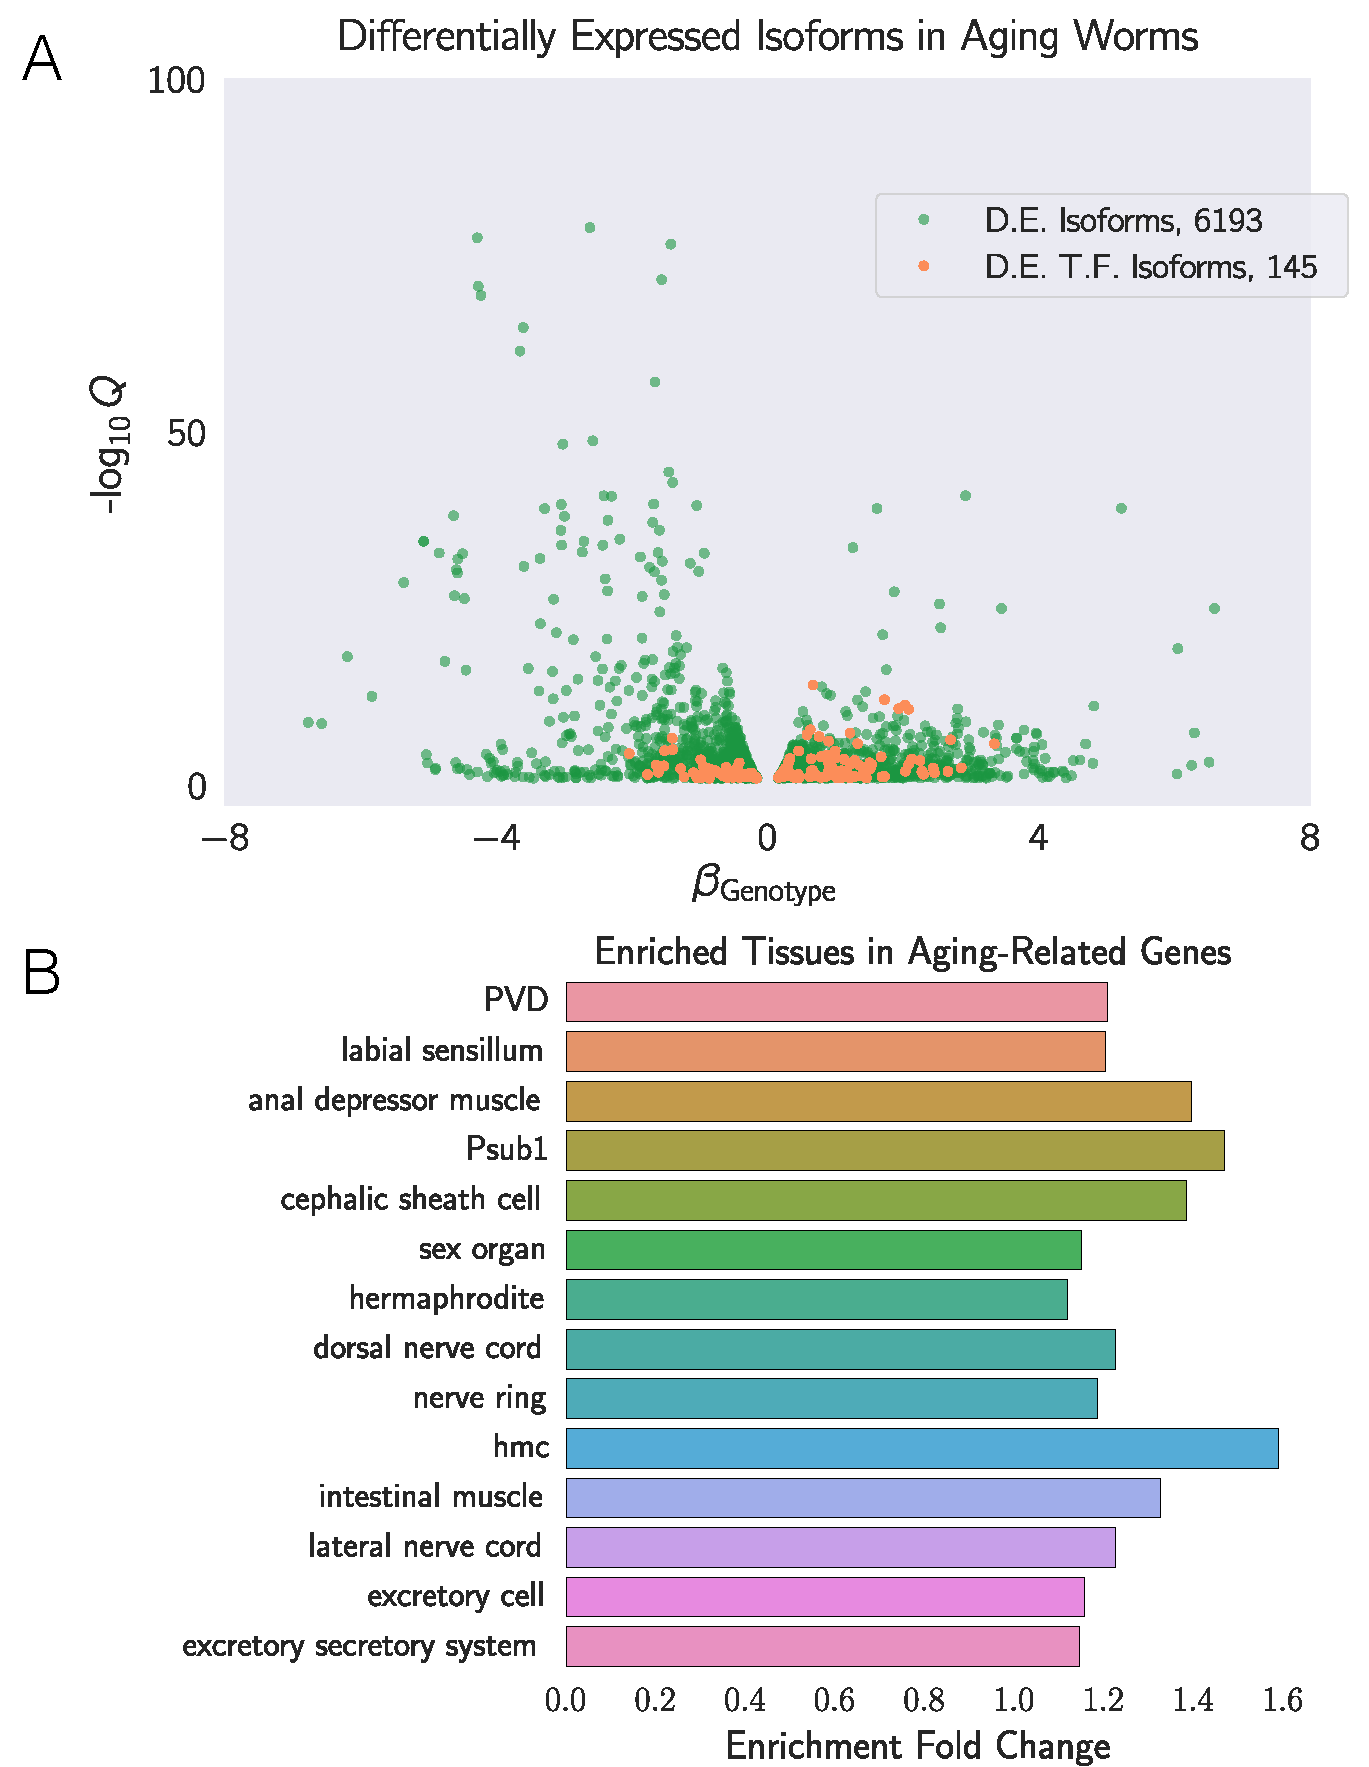
\includegraphics[width=\linewidth]{../../output/figs/final_figs/aging_transcriptomics.pdf}
  \caption{
    \textbf{A} We identified a common aging expression signature between N2 and
    \fog{} animals, consisting of 6,193 differentially expressed isoforms
    totaling \agen{} genes. The volcano plot is randomly down-sampled 30\% for
    ease of viewing. Each point represents an individual isoform.
    $\beta{}_\mathrm{Aging}$ is the regression coefficient. Larger magnitudes of
    $\beta$ indicate a larger log-fold change. The y-axis shows the negative
    logarithm of the q-values for each point. Green points are differentially
    expressed isoforms; orange points are differentially expressed isoforms of
    predicted transcription factor genes~\citep{Reece-Hoyes2005}. An interactive
    version of this graph can be found on our \webref{}. \textbf{B} Tissue
    Enrichment Analysis~\citep{Angeles-Albores2016} showed that genes associated
    with muscle tissues and the nervous system are enriched in aging-related
    genes. Only statistically significantly enriched tissues are shown.
    Enrichment Fold Change is defined as $Observed/Expected$.\ hmc stands for
    head mesodermal cell.
  }
\label{fig:agingtranscriptome}
\end{figure}

\subsection*{Decoupling time-dependent effects from sperm-status via general
linear models}
\label{sub:Transcriptomics}
In order to decouple time-dependent effects from changes associated with loss of
hermaphroditic sperm, we measured wild-type and \fog{} adults at the 1st day
adult stage (before visible embryos were present) and 6th day adult stage, when
all wild-type hermaphrodites have laid all their eggs (see
Fig~\ref{fig:wormlife}), but mortality is still low
($<10\%$)~\citep{Stroustrup2013}.  We obtained 16--19 million reads mappable to
the \cel{} genome per biological replicate, which enabled us to identify 14,702
individual genes totalling 21,143 isoforms (see
Figure~\ref{fig:agingtranscriptome}a).

\begin{figure}[htbp]
  \renewcommand{\familydefault}{\sfdefault}\normalfont{}
  \centering
  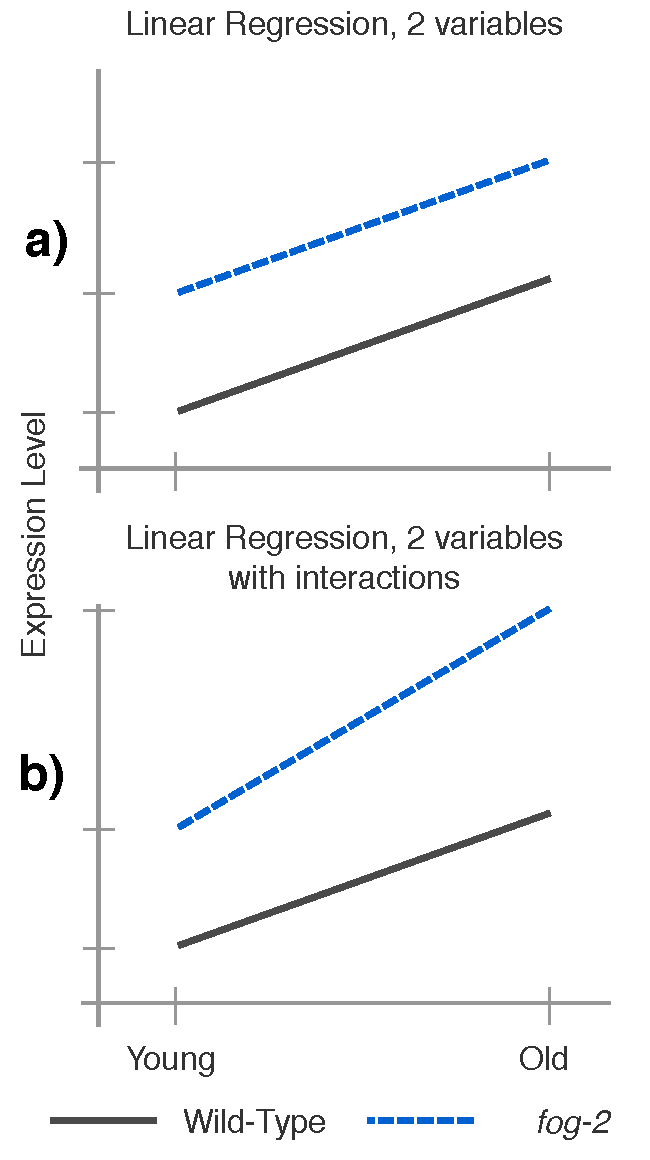
\includegraphics[width=\linewidth]{../../output/figs/final_figs/linear_regression.pdf}
  \caption{
    \textbf{A}. A linear regression with two variables, age and genotype. The
    expression level of a hypothetical gene increases by the same amount as
    worms age regardless of genotype. However, \fog{} has higher expression
    of this gene than the wild-type at all stages (blue arrow). \textbf{B}. A
    linear regression with two variables and an interaction term. In this
    example, the expression level of this hypothetical gene is different between
    wild-type worms and \fog{} (blue arrow). Although the expression level of
    this gene increases with age, the slope is different between wild-type and
    \fog{}. The difference in the slope can be accounted for through an
    interaction coefficient (red arrow).
  }
\label{fig:linear_reg}
\end{figure}

One way to analyze the data from this two-factor design is by pairwise
comparison of the distinct states. However, such an analysis would not make full
use of all the statistical power afforded by this experiment. Another method
that makes full use of the information in our experiment is to perform a linear
regression in 3 dimensions (2 independent variables, age and genotype, and 1
output). A linear regression with 1 parameter (age, for example) would fit a
line between expression data for young and old animals. When a second parameter
is added to the linear regression, said parameter can be visualized as altering
the y-intercept, but not the slope, of the first line in question (see
Fig.~\ref{fig:linear_reg}a).

Although a simple linear model is oftentimes useful, sometimes it is not
appropriate to assume that the two variables under study are entirely
independent. For example, in our case, three out of the four
timepoint-and-genotype combinations we studied did not have sperm, and
sperm-status is associated with both the \fog{} self-sterile phenotype and with
biological age of the wild-type animal. One way to statistically model such
correlation between variables is to add an interaction term to the linear
regression. This interaction term allows extra flexibility in describing how
changes occur between conditions. For example, suppose a given theoretical gene
\gene{X} has expression levels that increase in a \gene{fog-2}-dependent manner,
but also increases in an age-dependent manner. However, aged \fog{} animals do
not have the expression levels of \gene{X} that would be expected from adding
the effect of the two perturbations; instead, the expression levels of \gene{X}
in this animal are considerably above what is expected. In this case, we could
add a positive interaction coefficient to the model to explain the effect of
genotype on the y-intercept as well as the slope (see
Fig.~\ref{fig:linear_reg}b). When the two perturbations affect a single genetic
pathway, these interactions can be interpreted as epistatic interactions.

For these reasons, we used a general linear model with interactions to identify
a transcriptomic profile associated with the \fog{} genotype independently of
age, as well as a transcriptomic profile of \cel{} aging common to both
genotypes. The change associated with each variable is referred as $\beta$; this
number, although related to the natural logarithm of the fold change, is not
equal to it. However, it is true that larger magnitudes of $\beta$ indicate
greater change. Thus, for each gene we performed a linear regression, and we
evaluated the whether the $\beta$ values associated with each coefficient were
significantly different from 0 via a Wald test corrected for multiple hypothesis
testing. A coefficient was considered to be significantly different from 0 if
the q-value associated with it was less than 0.1.

\subsection*{A quarter of all genes change expression between the 1st day of
             adulthood and the 6th day of adulthood in \cel{}}
We identified a transcriptomic signature consisting of \agen{} genes that were
differentially expressed in 6th day adult animals of either genotype relative to
1st day adult animals (see SI file 2). This constitutes more than one quarter of
the genes in \cel{}. Tissue Enrichment Analysis
(TEA)~\citep{Angeles-Albores2016} showed that nervous tissues including the
`nerve ring', `dorsal nerve cord', `PVD' and `labial sensillum' were enriched in
genes that become differentially expressed through aging. Likewise, certain
muscle groups (`anal depressor muscle', `intestinal muscle') were enriched. (see
Figure~\ref{fig:agingtranscriptome}b). Gene Enrichment Analysis
(GEA)~\citep{Angeles-Albores106369} revealed that genes that were differentially
expressed during the course of aging were enriched in terms involving
respiration (`respiratory chain', `oxoacid metabolic process'); translation
(`cytosolic large ribosomal subunit'); and nucleotide metabolism (`purine
nucleotide', `nucleoside phosphate' and `ribose phosphate' metabolic process).
Phenotype Enrichment Analysis (PEA)~\citep{Angeles-Albores106369} showed this
gene list was associated with phenotypes that affect the \cel{} gonad, including
`gonad vesiculated', `gonad small', `oocytes lack nucleus' and `rachis narrow'.

To verify the quality of our dataset, we generated a list of \goldn{} golden
standard genes expected to be altered in 6th day adult worms using previous
literature reports including downstream genes of \gene{daf-12}, \gene{daf-16},
and aging and lifespan extension datasets~\citep{Murphy2003,
Halaschek-wiener2005,Lund2002,McCormick2012,Eckley2013}. Out of \goldn{}
standard genes, we found \goldfound{} genes in our time-responsive dataset. This
result was statistically significant with a p-value \goldpval{}.

Next, we used a published compendium~\citep{Reece-Hoyes2005} to search for known
or predicted transcription factors. We found \tfaging{} transcription factors in
the set of genes with differential expression in aging nematodes. We subjected
this list of transcription factors to TEA to understand their expression
patterns. 6 of these transcription factors were expressed in the `hermaphrodite
specific neuron' (HSN), a neuron physiologically relevant for egg-laying
(\gene{hlh-14}, \gene{sem-4}, \gene{ceh-20}, \gene{egl-46}, \gene{ceh-13},
\gene{hlh-3}), which represented a statistically significant 2-fold enrichment
of this tissue ($q<10^{-1}$). The term `head muscle' was also overrepresented at
twice the expected level ($q<10^{-1}$, 13 genes).

\subsection*{The whole-organism \fog{} differential expression signature}
We identified \fogn{} genes associated with the \fog{} genotype, including
\tffog{} transcription factors (see SI file 3). TEA showed that the terms `AB',
`somatic gonad', `uterine muscle', `cephalic sheath cell', `spermathecal-uterine
junction', and `PVD' were enriched in this gene set. The `somatic gonad' and
`spermathecal-uterine junction' are both near the site of action of \fog{} (the
germline) and possibly reflect physiological changes from a lack of sperm.
Phenotype ontology enrichment analysis showed that only a single phenotype term,
`spindle orientation variant' was enriched in the \fog{} transcriptional
signature ($q<10^{-1}$, 38 genes, 2-fold enrichment). Most genes annotated as
`spindle orientation variant' were slightly upregulated, and therefore are
unlikely to uniquely reflect reduced germline proliferation. GO term enrichment
was very similar to the aging gene set and reflected enrichment in annotations
pertaining to translation and respiration. Unlike the aging gene set, the \fog{}
signature was significantly enriched in `myofibril' and `G-protein coupled
receptor binding' ($q<10^{-1}$). Enrichment of the term `G-protein coupled
receptor binding' was due to 14 genes: \gene{cam-1}, \gene{mom-2},
\gene{dsh-1}, \gene{spp-10}, \gene{flp-6}, \gene{flp-7}, \gene{flp-9},
\gene{flp-13}, \gene{flp-14}, \gene{flp-18}, \gene{K02A11.4}, \gene{nlp-12},
\gene{nlp-13}, and \gene{nlp-40}. \gene{dsh-1}, \gene{mom-2} and \gene{cam-1}
are members of the Wnt signaling pathway. Most of these genes' expression levels
were up-regulated, suggesting increased G-protein binding activity in \fog{}
mutants.

\subsection*{The \fog{} expression signature overlaps significantly with the aging
signature}
Of the \fogn{} genes that we identified in the \fog{} signature, \intersectn{}
genes were also identified in our aging set. Moreover, of these \intersectn{}
genes, \coexpressed{} genes changed in the same direction in response to either
aging or germline feminization. The overlap between these signatures suggests an
interplay between sperm-status and age. The nature of the interplay should be
captured by the interaction coefficients in our model. There are four
possibilities. First, the \fog{} worms may have a fast-aging phenotype, in which
case the interaction coefficients should match the sign of the aging
coefficient. Second, the \fog{} worms may have a slow-aging phenotype, in which
case the interaction coefficients should have an interaction coefficient that is
of opposite sign, but not greater in magnitude than the aging coefficient (if a
gene increases in aging in a wild-type worm, it should still increase in a
\fog{} worm, albeit less). Third, the \fog{} worms exhibit a rejuvenation
phenotype. If this is the case, then these genes should have an interaction
coefficient that is of opposite sign and greater magnitude than their aging
coefficient, such that the change of these genes in \fog{} mutant worms is
reversed relative to the wild-type. Finally, if these genes are indicative of a
female-like state, then these genes should not change with age in \fog{} animals,
since these animals do not exit this state during the course of the experiment.
Moreover, because wild-type worms become female as they age, a further
requirement for a transcriptomic signature of the female-like state is that aging
coefficients for genes in this signature should have genotype coefficients of
equal sign and magnitude. In other words, entrance into the female-like state should
be not be path-dependent.


% aberrant aging
\begin{figure}
  \renewcommand{\familydefault}{\sfdefault}\normalfont{}
  \centering
  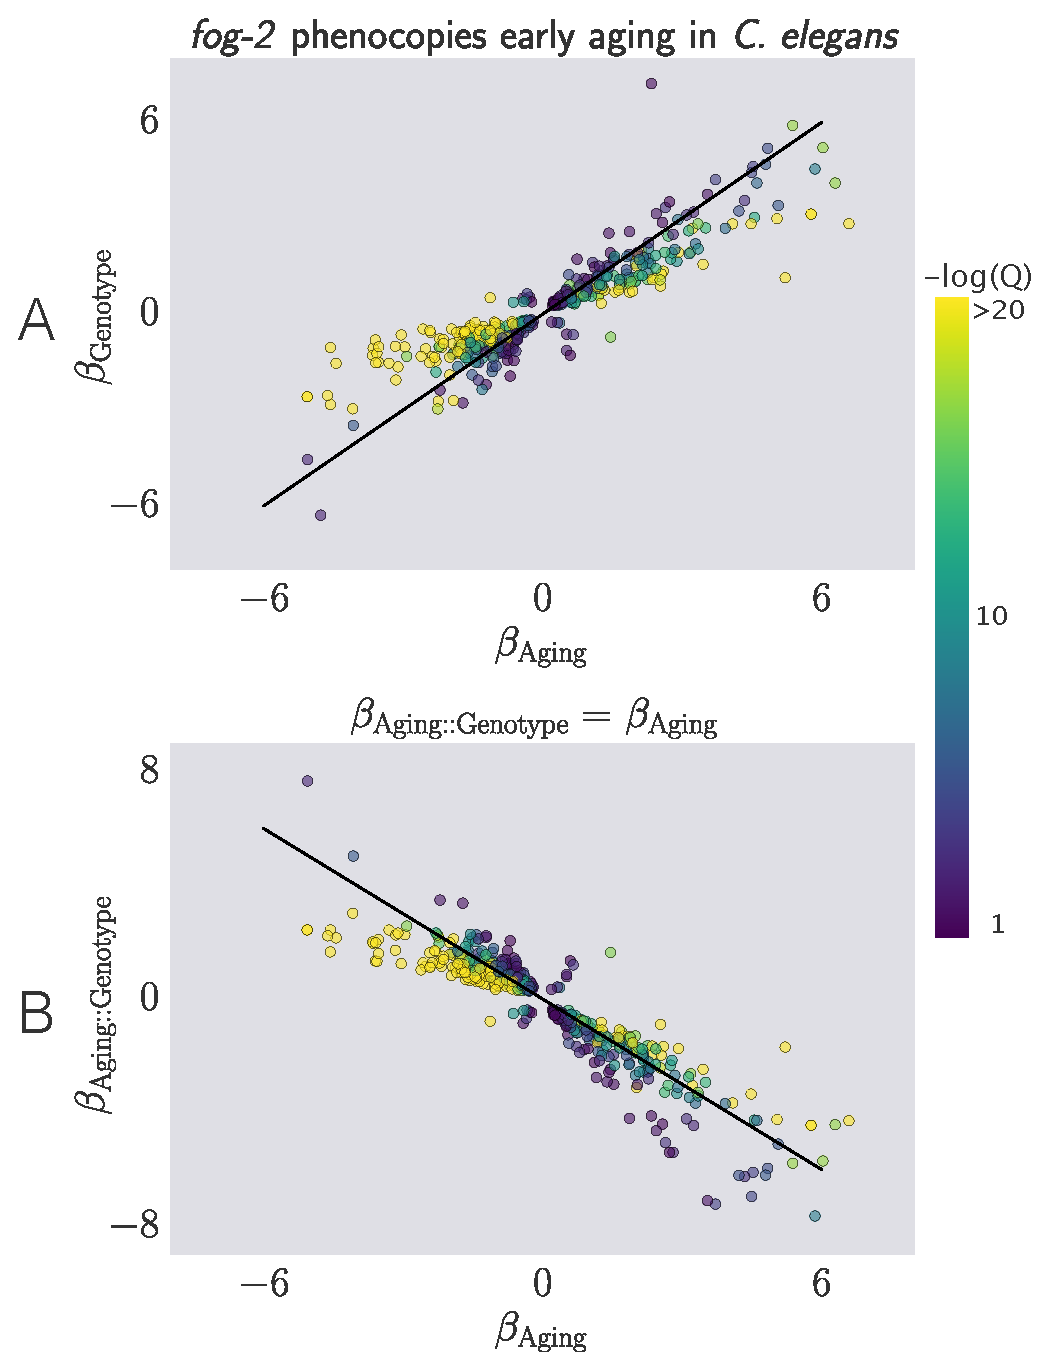
\includegraphics[width=\linewidth]{../../output/figs/final_figs/aberrant_aging.pdf}
  \caption{
    \fog{} partially phenocopies early aging in \cel{}. The $\beta$ in each axes
    is the regression coefficient from the GLM, and can be loosely interpreted
    as an estimator of the log-fold change. Feminization by loss of \fog{} is
    associated with a transcriptomic phenotype involving \fogn{} genes.
    \intersectn{}/\fogn{} of these genes are also altered in wild-type worms as
    they progress from young adulthood to old adulthood, and \coexpressed{}
    change in the same direction. However, progression from young to old
    adulthood in a \fog{} background results in no change in the expression
    level of these genes.
    \textbf{A} We identified genes that change similarly
    during feminization and aging. The correlation between feminization and
    aging is almost 1:1.
    \textbf{B} Epistasis plot of aging versus feminization.
    Epistasis plots indicate whether two genes (or perturbations) act on the
    same pathway. When two effects act on the same pathway, this is reflected by
    a slope of $-0.5$. The measured slope was $-0.51 \pm 0.01$.
  }%
\label{fig:aberrant_aging}
\end{figure}

To evaluate which of these possibilities was most likely, we selected the
\intersectn{} genes that had aging, genotype and interaction coefficients
significantly different from zero and we plotted their temporal coefficients
against their genotype coefficients (see Fig.~\ref{fig:aberrant_aging}a). We
observed that the aging coefficients were strongly predictive of the genotype
coefficients. Most of these genes fell near the line $y=x$, suggesting that
these genes define a female-like state.

We considered how loss-of-function of \gene{fog-2} and aging could both interact
to cause entry into this state. We reasoned that a plausible mechanism is that
\gene{fog-2} promotes sperm-production, and aging promotes sperm-depletion. This
simple pathway model suggests that a double perturbation consisting of aging and
loss of function of \gene{fog-2} should show non-additivity of phenotypes
(generalized epistasis). To test whether these two perturbations deviate from
additivity, we generated an epistasis plot using this gene set. We
have previously used epistasis plots to measure transcriptome-wide epistasis
between genes in a pathway~\citep{Angeles-Albores2017}. Briefly, an epistasis
plot shows the expected expression of a double perturbation under an additive
model (null model) on the x-axis, and the deviation from this null model in the
y-axis. In other words, we calculated the x-coordinates for each point by adding
$\beta_\mathrm{Genotype} + \beta_\mathrm{Aging}$, and the y-coordinates are
equal to $\beta_{Interaction}$ for each isoform. Previously we have shown that
if two genes or perturbations act within a linear pathway, an epistasis plot
will generate a line with slope equal to $-0.5$. When we generated an epistasis
plot and found the line of best fit, we observed a slope of $-0.51\pm 0.01$,
which suggests that the \gene{fog-2} gene and time are acting to generate a
single transcriptomic phenotype along a single pathway. Overall, we identified
\femalen{} genes that changed in the same direction through age or mutation of
the \fog{} gene and that had an interaction coefficient of opposite sign to the
aging or genotype coefficient (see SI file 4). Taken together, this information
suggests that these \femalen{} genes define a female-like state in \cel{}.

\subsection*{Analysis of the female-like state expression signature}

\begin{figure}
  \renewcommand{\familydefault}{\sfdefault}\normalfont{}
  \centering
  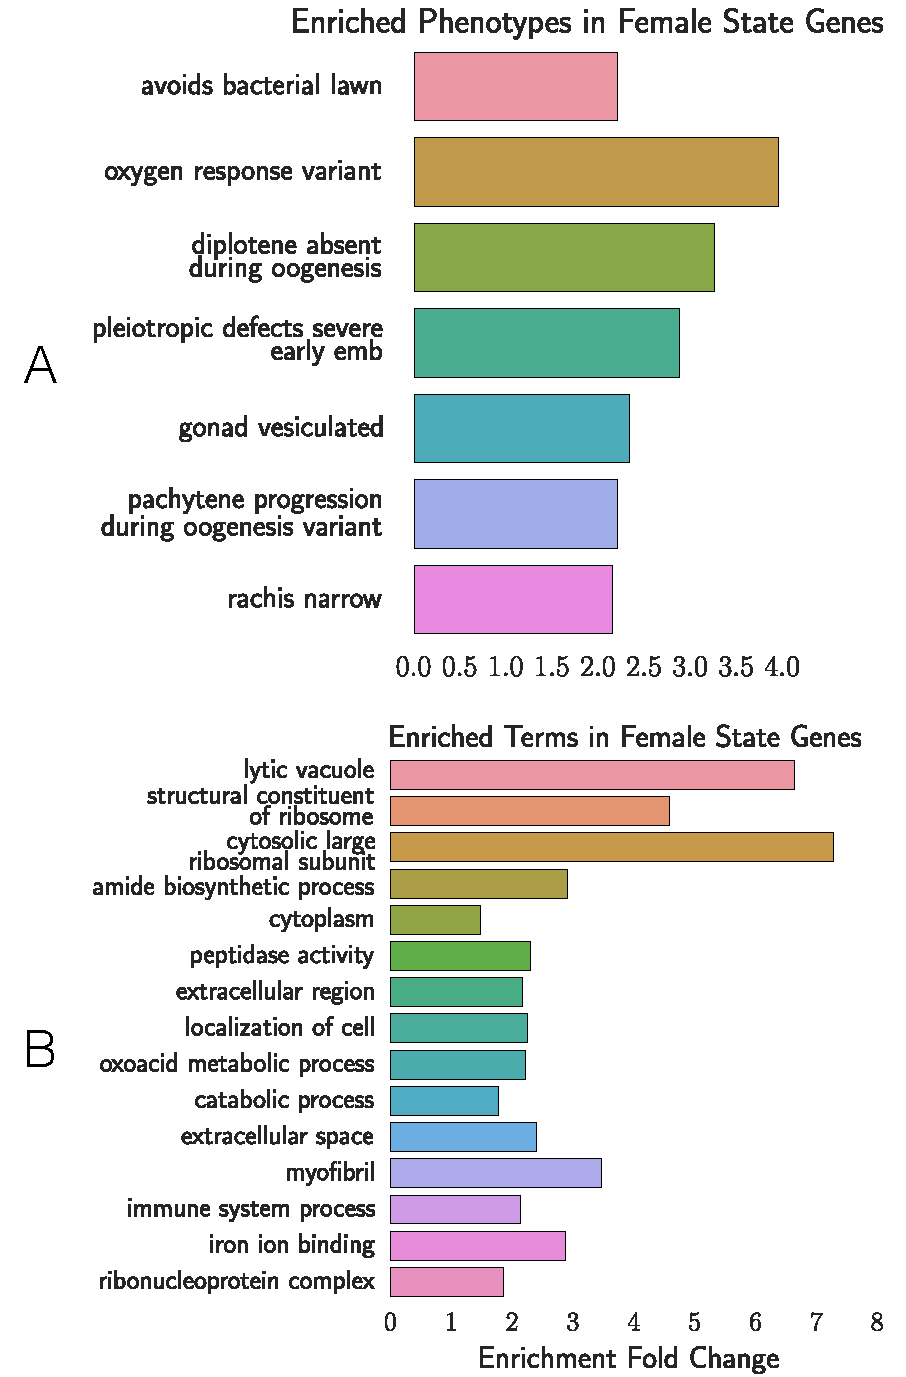
\includegraphics[width=0.9\linewidth]
  {../../output/figs/final_figs/female_state_enrichment.pdf}
  \caption{
    Phenotype and GO enrichment of genes involved in the female-like state.
    \textbf{A}. Phenotype Enrichment Analysis.
    \textbf{B}. Gene Ontology Enrichment Analysis.
    Most of the terms enriched in PEA reflect the abundance of ribosomal subunits
    present in this gene set.
  }
\label{fig:female_state_enrich}
\end{figure}

To better understand the changes that happen after sperm loss, we performed
tissue enrichment, phenotype enrichment and gene ontology enrichment analyses on
the set of \femalen{} genes that we associated with the female-like state. TEA showed
no tissue enrichment using this gene-set. GEA showed that this gene list was
enriched in constituents of the ribosomal subunits almost four times above
background ($q<10^{-5}$, 17 genes). The enrichment of ribosomal constituents in
this gene set in turn drives the enriched phenotypes: `avoids bacterial lawn',
`diplotene absent during oogenesis', `gonad vesiculated', `pachytene progression
during oogenesis variant', and `rachis narrow'. The expression of most of these
ribosomal subunits is down-regulated in aged animals or in \fog{} mutants.

\section{Discussion}
\label{sec:discussion}

\subsection*{Defining an Early Aging Phenotype}
\label{sub:Defining an Early Aging Phenotype}

Our experimental design enables us to decouple the effects of egg-laying from
aging. As a result, we identified a set of almost 4,000 genes that are altered
similarly between wild-type and \fog{} mutants. Due to the read depth of our
transcriptomic data (20 million reads) and the number of samples measured (3
biological replicates for 4 different life stages/genotypes), this dataset
constitutes a high-quality description of the transcriptomic changes that occur
in aging populations of \cel{}. Although our data only capture $\sim50\%$ of the
expression changes reported in earlier aging transcriptome literature, this
disagreement can be explained by a difference in methodology; earlier
publications typically addressed the aging of fertile wild-type hermaphrodites
only indirectly, or queried aging animals at a much later stage of their life
cycle.


\subsection*{General linear models enable epistasis measurements}
\label{sub:lin_models}

We set out to study the self-fertilizing (hermaphroditic) to self-sterile
(female-like) transition by comparing wild-type animals with \fog{} mutants as
they aged. Our computational approach enabled us to separate between two
biological processes that are correlated within samples. Because of this
intra-sample correlation, identifying this state via pairwise comparisons would
not have been straightforward. Although it is a favored method amongst
biologists, such pairwise comparisons suffer from a number of drawbacks. First,
pairwise comparisons are unable to draw on the full statistical power available
to an experiment because they discard almost all information except the samples
being compared. Second, pairwise comparisons require a researcher to define
\emph{a priori} which comparisons are informative. For experiments with many
variables, the number of pairwise combinations is explosively large. Indeed,
even for this two-factor experiment, there are 6 possible pairwise comparisons.
On the other hand, by specifying a linear regression model, each gene can be
summarized with three variables, each of which can be analyzed and understood
without the need to resort to further pairwise combinations.

\subsection*{The \cel{} female-like state}
\label{sub:female_state}
Our explorations have shown that the loss of \fog{} partially phenocopies the
transcriptional events that occur naturally as \cel{} ages from the 1st day of
adulthood to the 6th day of adulthood. Moreover, epistasis analysis of these
perturbations suggest that they act on the same pathway, namely sperm generation
and depletion (see Fig.~\ref{fig:lifecycle}). Self-sperm generation promotes the
hermaphrodite state, whereas sperm depletion marks entry into the female-like
state. Given the enrichment of neuronal transcription factors that are
associated with sperm loss in our dataset, we believe this dataset should
contain some of the transcriptomic modules that are involved in these pheromone
production and behavioral pathways, although we have been unable to find these
genes.

Behavioral and physiological changes upon mating are not unknown in other
species. In particular, in the fruit fly \emph{Drosophila melanogaster}, sex
peptide present in the male seminal fluid is known to drive changes in gene
expression~\citep{Liu2003,Xue2000,Avila2011} as well as behavior. More recently,
sperm was found to be necessary to drive changes in aggression in the fruit
fly~\citep{Bath2017}. These changes are often reversible upon the disappearance
of seminal fluid or sperm. In the case of \cel{}, we have observed that sperm
loss is associated with gene expression changes that probably reflect
physiological changes in the worm. Our experimental design did not include a
test for reversibility of these changes. The possibility of a rescue experiment
with males raises interesting possibilities: What fraction of the changes
observed upon loss of self-sperm are reversible? Do male seminal fluid or male
sperm cause changes beyond rescue?

\subsection*{The \cel{} life cycle, life stages and life states}

\begin{figure}
  \renewcommand{\familydefault}{\sfdefault}\normalfont{}
  \centering
  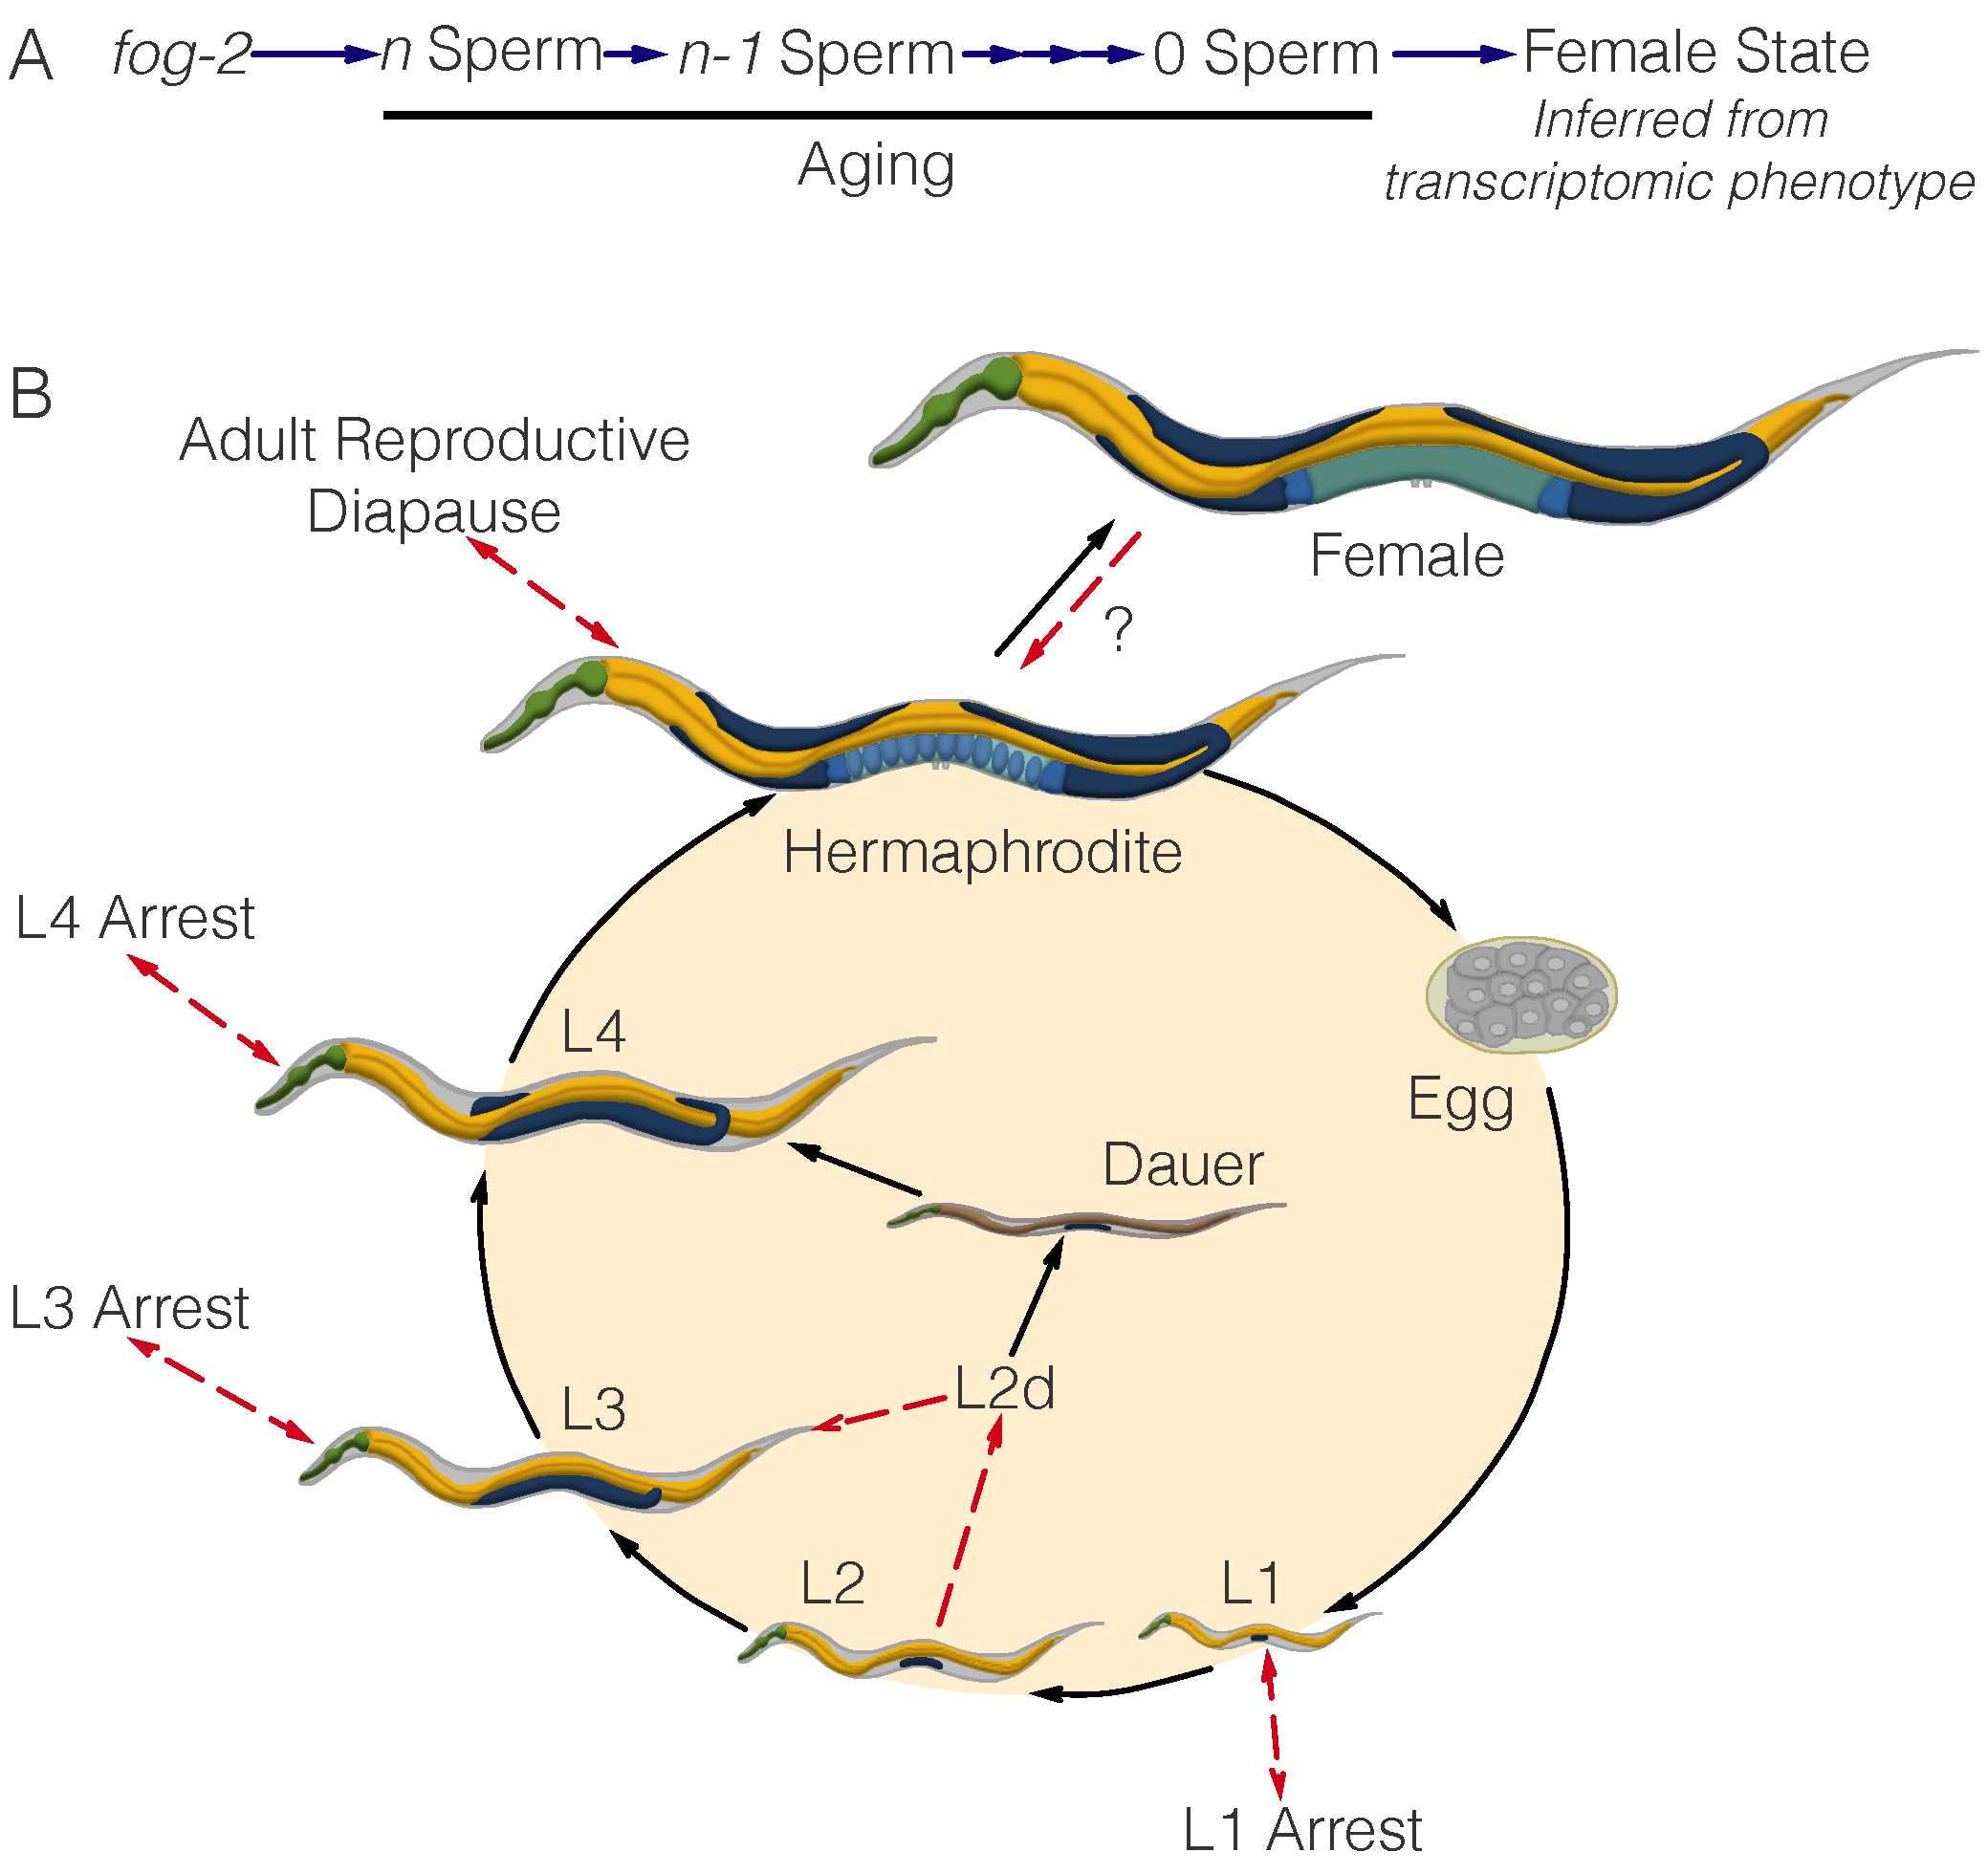
\includegraphics[width=\linewidth]{../../output/figs/final_figs/c_elegans_life_cycle.pdf}
  \caption{
    \textbf{A}. A substrate model showing how \gene{fog-2} promotes sperm
    generation, whereas aging promotes sperm depletion, leading to entry to the
    female-like state. Such a model can explain why \gene{fog-2} and aging appear
    epistatic to each other.
    \textbf{B}. The complete \cel{} life cycle.
    Recognized stages of \cel{} are marked by black arrows. States are marked by
    red arrows to emphasize that at the end of a state, the worm returns to the
    developmental timepoint it was at before entering the state. The L2d state
    is an exception. It is the only stage that does not return to the same
    developmental timepoint; rather, the L2d state is a permissive state that
    allows entry into either dauer or the L3 stage. We have presented evidence
    of a female-like state in \cel{}. At this point, it is unclear whether the
    difference between hermaphrodites and females is reversible by males.
    Therefore, it remains unclear whether it is a stage or a true state.
  }%
\label{fig:lifecycle}
\end{figure}

\cel{} has a complicated life cycle, with two alternative developmental pathways
that have multiple stages (larval development and dauer development), followed
by reproductive adulthood. In addition to its developmental stages, researchers
have recognized that \cel{} has numerous life states that it can enter into when
given instructive environmental cues. One such state is the L1 arrest state,
where development ceases entirely upon starvation~\citep{Johnson1984}. More
recently, researchers have described additional diapause states that the worm
can access at the L3, L4 and young adult stages under conditions of low
food~\citep{Angelo2009,Seidel2011,Schindler2014}. Not all states of \cel{} are
arrested, however (see Fig.~\ref{fig:lifecycle}). For example, the L2d state is
induced by crowded and nutrient poor conditions~\citep{Golden1984}. While within
this state, the worm is capable of entry into either dauer or the L3 larval
stage, depending on environmental conditions. Thus, the L2d state is a
permissive state, and marks the point at which the nematode development is
committed to a single developmental pathway.

Identification of the \cel{} life states has often been performed by
morphological studies (as in the course of L4 arrest or L2d) or via timecourses
(L1 arrest). However, not all states may be visually identifiable, or even if
they are, the morphological changes may be very subtle, making positive
identification difficult. However, the detailed information afforded by a
transcriptome should in theory provide sufficient information to definitively
identify a state, since transcriptomic information underlies morphology.
Moreover, transcriptomics can provide an informative description into the
physiology of complex metazoan life state's. By identifying differentially
expressed genes and using ontology enrichment analyses to identify gene
functions, sites of expression or phenotypes that are enriched in a given gene
set, we can obtain a clear picture of the changes that occur in the worm
analogous to identifying gross morphological changes.

RNA-seq is a powerful technology that has been used successfully in the past as
a qualitative tool for target acquisition, though recent work has successfully
used RNA-seq to measure genetic interactions via
epistasis~\citep{Dixit2016,Angeles-Albores2017}. Here, we have shown that
whole-organism RNA-seq data can also be used to successfully identify internal
states in a multi-cellular organism.

% \subsection*{mRNA Levels of Developmental Factors Change Between 1st
%              to 6th Day of Adulthood in \cel{}}
% \label{sub:development_in_aging}
%
% Our transcriptomes reveal a host of transcription factors that changed between
% the 1st and 6th day of adulthood in \cel{}. Many of these transcription factors
% have been associated with development via cellular differentiation and
% specification. For example, we identified the transcription factor
% \emph{lin-32}, which has been associated with neuron
% development~\citep{Chalfie1989,Zhao1995,Portman2000}; the Six5 ortholog
% \emph{unc-39} has been associated with axonal pathfinding and neuron
% migration\citep{Manser1990,Yanowitz2004}; \emph{cnd-1}, a homolog  of the
% vertebrate NeuroD transcription factors, is expressed in the early embryo and is
% also involved in axon guidance~\citep{Schmitz2007}.
% Why these transcription factors increase their expression is a mystery,
% but we speculate that this hints at important neuronal changes that are
% taking place.


\section*{Acknowledgments}

We thank the \emph{Caenorhabditis} Genetics Center for providing worm strains.
This work would not be possible without the central repository of \cel{}
information generated by WormBase, without which mining the genetic data would
not have been possible. DHWL was supported by a National Institutes of Health US
Public Health Service Training Grant (T32GM07616). This research was supported
by the Howard Hughes Medical Institute, for which PWS is an investigator.

\subsubsection*{Author Contributions:}
DA, DHWL and PWS designed all experiments. DHWL and THK collected RNA for
library preparation. IA generated libraries and performed sequencing. DA
performed all bioinformatics and statistical analyses. DA, TT and DHWL performed
all screens. DA, DHWL and PWS wrote the paper.



\bibliography{citations}

\end{document}
